\chapter{Section 2:  Seasons and Calendars across cultures}
The purely qualitative methods, results, and interpretive discussion.

\section{Methods}
Qualitative; snowball interview recruitment with three 'seeds' (Yolngu, UCA, Science).
Reflecting on results, it's more complex than I first thought.

\section{Results and Discussion}
'Calendar' and 'season' are not concepts that translate directly across cultures. 
Discuss how I realised this, by re-listening to recordings, and that I was expecting something unforeseen (but not like this!).  
Yolngu participants discussed three levels of seasons:  wet-dry, 'the six', and the many.

\begin{figure}[h]
    \centering
    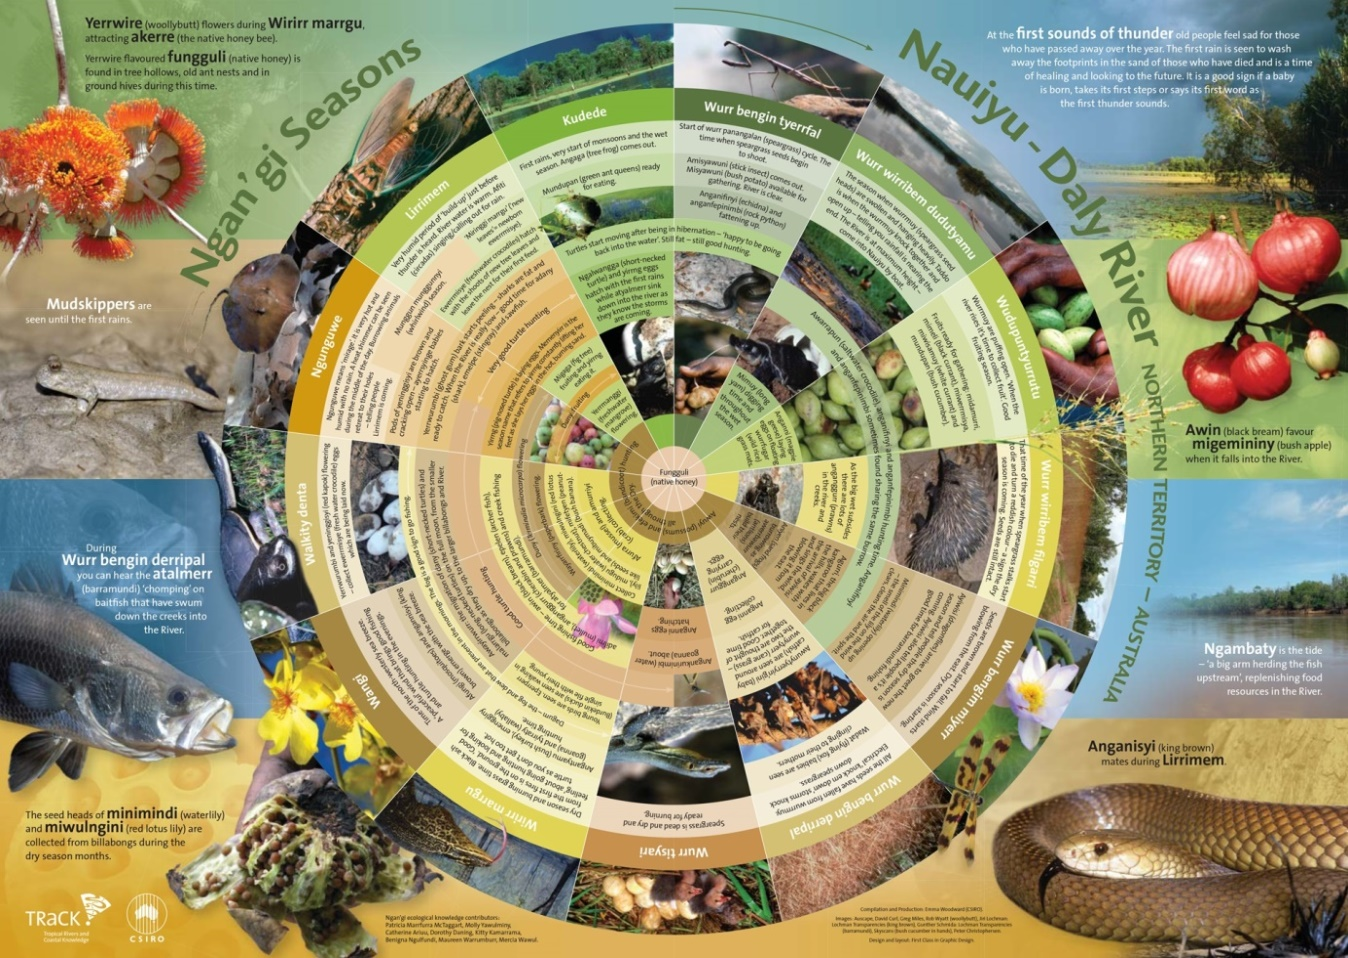
\includegraphics[width=0.8\textwidth]{ngangi-calendar.jpg}
    \caption{An indigenous seasonal calendar, for Ngan'gi seasons \citep{CSIROcals}}
    \label{fig:ngangi-seasons}
\end{figure}

Use TRaCK poster to highlight the six and many seasons (each box a microseason).
The two are <give some detail or quotes>.
The six are <>.
Completeness of the many is out of scope, but <examples>.  

For the remainder of this thesis I'll focus on the six, which best facilitates knowledge synthesis.

